%Multi gnss
%Segments
%Stopwatch
%Code tracking loop thing?

%What is gnss? %which systems exist? %Which are operational? %Will focus on gps here
A Global Navigation Satellite System, is a navigation system that provides position solutions from radio signals transmitted by orbiting satellites \cite{groves2013principles}. This is a collective term for several existing systems, as of March 2019, the American GPS, the Russian GLONASS, the European Galileo and the Chinese BeiDou. The two latter of which are still under development, expected to be operational in 2020, but currently offers partial coverage \cite{galOper, beidouGlob}. Additionally, several regional augmentation systems that are compatible with GNSS exist. The following chapter will focus on GPS as it is arguably the most well known system. \\

GNSS is split into three \textit{segments}:

\begin{itemize}
\item Space segment: Composed of all satellites, also called satellite vehicles (SV), in orbit transmitting GNSS data.
\item Control segment: Monitors and updates the clock correction and orbital parameters of each satellite.
\item User segment: Composed of all GNSS-receivers. Both military, civilian and commercial.
\end{itemize}

%How does it work? (in short)
The satellites of each GNSS keep a medium Earth orbit, with the exception of some geostationary Beidou satellites in a geostationary orbit. These orbits gives a better signal geometry, yielding a more precise navigation solution, and better coverage in polar regions \cite{groves2013principles}. Each satellite is closely monitored by a number of control stations spread around the planet, that periodically uploads precise orbital parameters to the satellites. In turn the satellites continuously broadcast said parameters to the receivers of the user segments, along with the time of transmission. The receiver may then calculate the satellite's position from the orbital parameters, as well as the range to the transmitting satellite as signal travel time multiplied by the speed of light. From this it is possible to estimate the user's position as indicated in figure \ref{fig:pos-est}. However, as errors are multiplied by the speed of light, this is only made possible by a set of extremely precise atomic clocks onboard each satellite. The triangulation concept is shown in figure \ref{fig:pos-est}.

%\missingfigure[]{Position estimation from geogebra maybe}
\begin{figure}
    \centering
    \definecolor{qqffqq}{rgb}{0,1,0}
\definecolor{ffqqqq}{rgb}{1,0,0}
\definecolor{qqqqff}{rgb}{0,0,1}

\begin{tikzpicture}[line cap=round,line join=round,>=triangle 45,x=1cm,y=1cm]
\clip(-4.774627483569065,-3.838278779077957) rectangle (6.50099294588812,6.9559114583626425);
\draw [line width=2pt,dash pattern=on 1pt off 1pt,color=qqqqff] (-1.4092642007055942,-1.4048037632482042) circle (1.9898490396577058cm);
\draw [line width=2pt,dash pattern=on 1pt off 1pt,color=ffqqqq] (2.5582442445802016,0) circle (2.5582442445802016cm);
\draw [line width=2pt,dash pattern=on 1pt off 1pt,color=qqffqq] (-1.2049290018067518,2.273229816930906) circle (2.5728248482900535cm);
\draw [line width=2pt] (2.5582442445802016,0)-- (0,0);
\draw [line width=2pt] (-1.4092642007055942,-1.4048037632482042)-- (0,0);
\draw [line width=2pt] (0,0)-- (-1.2049290018067518,2.273229816930906);
\begin{scriptsize}
\draw [fill=uuuuuu] (0,0) circle (2pt);
\draw[color=uuuuuu] (0.552044109937058,0.2979895609087916) node {$Receiver$};
\draw [fill=ududff] (-1.4092642007055942,-1.4048037632482042) circle (2.5pt);
\draw[color=ududff] (-1.1662291535304545,-1.079725037727322) node {$SV3$};
\draw [fill=xdxdff] (2.5582442445802016,0) circle (2.5pt);
\draw[color=xdxdff] (2.812115249272705,0.3289494395298278) node {$SV2$};
\draw [fill=ududff] (-1.2049290018067518,2.273229816930906) circle (2.5pt);
\draw[color=ududff] (-0.9649899424937187,2.604500518175993) node {$SV1$};
\draw[color=black] (2.100038040988871,0.31346950021930975) node {$r2$};
\draw[color=black] (-0.9649899424937187,-0.6772466156538506) node {$r3$};
\draw[color=black] (-0.7637507314569831,2.000782885065786) node {$r1$};
\end{scriptsize}
\end{tikzpicture}
    \caption[Triangulation principle]{This figure illustrates the concept of triangulation from set of satellites, neglecting any measurement errors. SV1-SV3 denotes a set of satellites, while r1-r3 denotes the distance between them and the receiver. Circles with radii given by the ranges are also shown, and the receiver position is given by the intersection of these.}
    \label{fig:pos-est}
\end{figure}

\subsection{Signal composition}
GPS is currently undergoing a modernization program, replacing the old, \textit{legacy}, signals \cite{groves2013principles, farrell2008aided}. However, as these have not been fully introduced yet, this thesis will focus on the legacy civillian L1 C / A signal. This signal consists of three distinct parts; the carrier frequency of 1575.42 MHz, a \textit{pseudo-random noise} sequence and a navigation message \cite{misra2006global}. 

\subsubsection{Pseudo random noise codes}
The pseudo-random noise, also known as a PRN code or C/A code for the L1 signal, is a sequence of 1023 bits, repeated each millisecond. They are unique to each satellite, and have interesting properties with regard to both auto- and cross-correlation as distinct codes are nearly orthogonal to each other. In other words, the cross-correlation of two distinct, arbitrarily shifted, PRN-codes is nearly zero, meaning that satellites can broadcast simultaneously at the same frequency with no risk of interfering with each other. This is known as code-division multiple access (CDMA) \cite{groves2013principles}. The other property is that the auto-correlation, correlating a PRN code with itself, peaks for an unshifted code sequence. This allows a receiver to align a replica of a PRN code with an incoming one, and thus establish a common time reference. Figure \ref{fig:prn-match} illustrates this concept.\\

\begin{figure}[!htbp]
    \centering
    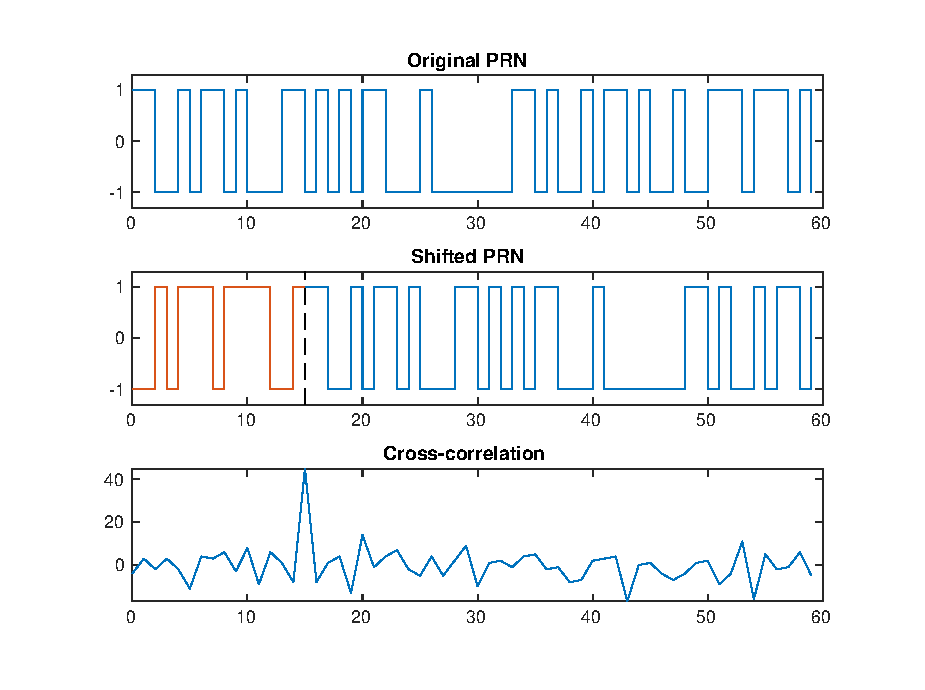
\includegraphics[scale=0.7]{bilder/prn_autocorr.eps}
    \caption{Cross-correlation between a PRN code shifted by 15 bits and the original unshifted sequence.}
    \label{fig:prn-match}
\end{figure}

\subsubsection{Navigation message}
The navigation message includes orbital parameters for calculating satellite position and velocity and is usually called the \textit{ephemeris}. It also contains satellite clock error parameters and the \textit{almanac}, a coarse ephemeris that allows a receiver to calculate the approximate positions of all satellites. This is used to predict when a satellite might be visible and aids rapid signal acquisition \cite{misra2006global}, see section \ref{sec:pr}. The almanac has a longer lifespan than the ephemeris, estimating satellite positions to an accuracy of 3600 meters up to two weeks after the initial upload \cite{groves2013principles}, and is often stored in the receiver between shutdowns. Additionally, the almanac includes parameters from the Klobuchar ionospheric model, described in appendix \ref{app:klobuchar}. The ephemeris and clock error equations are described in detail in section \ref{sec:ephemeris}.
    
\subsection{Observables}
\subsubsection{Pseudo-range} 
\label{sec:pr}
%Acquisition
When a receiver detects the signal of a new satellite, it will try to lock on to it. This is the process of initially aligning the replica PRN code to that of an incoming signal, and is known as signal \textit{acquisition}. When a match is found for a given signal, and hence the signal phase determined, it is assigned a channel in the receiver, and the \textit{code tracking} process can begin. This is were the pseudo-range measurements comes from; an incoming acquired signal will have lagged behind the replica PRN during the time of transmission, and multiplying the lag time by the speed of light, the pseudo-range is found. \\

The measurement is called \textit{pseudo}-range as it incorporates numerous errors with the true range, and are explained in more detail in section \ref{sec:errors}. This includes both satellite and receiver clock errors, atmospheric delays and relativistic effects as well as others, shown in figure \ref{fig:pr-delay}. The pseudo-range between the receiver and a satellite can be modeled as follows \cite{farrell2008aided}
\begin{align}
    P &= \rho + \beta - c\Delta t_{sv} + I_r + T_r + \delta p_{sagnac} + \vartheta\\
    \label{eq:pr-model}
    \intertext{Where $\rho$ is the geometric range, $\beta$ is the receiver clock error scaled by the speed of light, $\Delta t_{sv}_i$ the satellite clock error, $I_{r_i}$ the ionospheric delay, $T_{r}$ the tropospheric delay and $\vartheta$ are the unmodeled errors. The geometric range is given by}
    \rho &= \norm{\bm{p}_r - \bm{p}_s}_2 = \sqrt{(x_r - x_s)^2 + (y_r - y_s)^2 + (z_r - z_s)^2}
    \intertext{With $\bm{p}_r$ being the receiver position at the time of reception and $\bm{p}_s$ the satellite position at the time of transmission.}
\end{align}

\missingfigure[]{pseudo-range}
\begin{figure}
    \centering
    \includegraphics{}
    \caption{Pseudo-range with errors}
    \label{fig:pr-delay}
\end{figure}

\todo{Directly observable brukt riktig?}
\todo{Mention position estimation 4 sat?}
%receiver clock bias

\subsubsection{Doppler shift}
\missingfigure[]{Doppler shift}
% Acquisition requires known doppler, or search through frequency
During satellite acquisition, the high velocity difference of satellite and receiver introduces a Doppler shift on the carrier wave frequency. Hence, if the Doppler shift is unknown or cannot be otherwise estimated, the acquisition process requires a search along frequency in addition to phase. After acquisition, a rough estimate of the Doppler shift has been found and the receiver starts tracking further changes in the incoming carrier wave frequency. Taking advantage of the fact that the relative motion of satellite and receiver is far below the wave propagation speed, the received frequency is approximated as (\cite{li2011doppler, groves2013principles})
\begin{align}
    f_{received} &= 1 - \frac{(\bm{v}^e_{is} - \bm{v}^e_{ir}) \cdot \bm{l}^e_ {r,s}}{c}f_{transmitted}\\
    %
    \intertext{Where $\bm{l}^e_ {r,s}$ is the line of sight vector between satellite and receiver. Consequently the Doppler shift is}
    %
    \Delta f &= f_{received} - f_{transmitted} = -\frac{(\bm{v}^e_{is} - \bm{v}^e_{ir}) \cdot \bm{l}^e_ {r,s}}{c}f_{transmitted}
    %
    \intertext{Multiplying by the transmitted signal wavelength yields the relationship between the range rate and the Doppler shift as}
    %
    \dot{\range} &= -\lambda\Delta f = (\bm{v}^e_{is} - \bm{v}^e_{ir}) \cdot \bm{l}^e_ {r,s}
    \label{eq:range-rate}
    %
    \intertext{Where $\lambda$ is the wavelength of the transmitted signal. The model for the pseudo-range rate is}
    \dot{\pr} &= \dot{\rho} + \dot{\beta} - c\Delta \dot{t}_{{sv}} + \dot{I}_r + \dot{T}_r + \delta \dot{p}_{sagnac} + \dot{\vartheta}
    %
    \intertext{However, $\Delta t_{sv}$, $I_r$ and $T_r$ are slowly time varying \cite{farrell2008aided}, simplifying the model to}
    %
    \dot{\pr} &= \dot{\range} + \dot{\beta} + \delta \dot{p}_{sagnac} + \dot{\vartheta}
    \label{eq:prr-model}
\end{align}
where $\dot{\vartheta}_i$ represents the drift of any unmodeled errors.\\

\todo{switch out i subscript with s}
\todo{Add to nomenclature}
As the doppler measurement is dependent on receiver velocity, it can be applied to the navigation filter to yield a directly observed receiver velocity estimate. It is also dependent on the line of sight vector, and therefore position, but this dependence is weak \cite{misra2006global, groves2013principles}, and Doppler positioning is rarely used in GNSS position. A weighted least squares approach to PV-estimation is shown in \cite{li2011doppler}, based on pseudo-range and doppler measurements. \cite{shames2011analysis, shames2013doppler} makes an analytical analysis of the number of required measurements for PV-estimation in two dimensions, but states that it is easily generalized to three, albeit with the assumption that measurements are unbiased.

\subsubsection{Carrier Phase}
The carrier phase measurement will only be mentioned briefly in this thesis, as it has not been used explicitly in the implemented navigation filter. Nonetheless, as these measurements were readily available with the pseudo-range and doppler shift measurements, they were still included in the internal message bus of the system, and is considered a possibility for future additions.\\

The low noise of the carrier phase measurement can be taken advantage of by being integrated into a pseduo-range filter. This is known as carrier smoothing and one example is the recursive \textit{Hatch} filter \cite{misra2006global}
\begin{equation}
    \Bar{P}_n = \frac{1}{M}P_n + \frac{M-1}{M}(\Bar{P}_{n-1} + \Phi_n - \Phi_{n-1})
\end{equation}
Where $\Bar{P}_n$ is the smoothed pseudo-range of iteration n and $\Phi_n$ is the carrier phase measurement given in meters.\\

Carrier phase can also be used to improve velocity estimates. By using time-differenced carrier phase measurements, velocity can be estimated within the order of mm/s, as opposed to the Doppler approach with a resolution in the order of cm/s. This approach is explained further in \cite{freda2015time}. \cite{hansen2018nonlinear} also includes this measurement with a nonlinear observer.

%Mentioned for completeness, not used in this thesis
%Carrier smoothing

\subsection{Ephemeris calculations}
\label{sec:ephemeris}
The ephemeris and clock correction parameters as well as the accompanying equations are shown in table \ref{tab:ephemeris} and equation set \ref{eq:ephemeris}, respectively. Satellite velocities are needed to estimate receiver velocity from the doppler shift, but the equations are not shown here. \cite{zhang2006gps} derives equations for calculating satellite velocity, but concludes that a simple two point numerical differentiation is precise to the order of millimeters. As opposed to the other GNSS, GLONASS does not broadcast any Keplerian parameters, rather broadcasting ECEF position, velocity and acceleration directly. \cite{groves2013principles}\\
%The latter approach is used by RTKLIB (section \ref{sec:rtklib}) and consequently in this thesis as well.

\subsubsection{Ephemeris equations}
\todo{Move to appendix}
\label{sec:eph_equations}
\begin{table}[!htbp]
\noindent
\textbf{Time}\\
\begin{tabular}{l r}
	\begin{tabular}{l | r}
	\multicolumn{2}{l}{\textit{Parameters}}\\
	\hline
	$t_{sv}$ & Satellite broadcast time \\
	$w_n$ & Satellite week \\
	$t_{ow}$ & Seconds in GPS week \\
	$t_{gd}$ & Group delay \\
    $t_{oc}$ & Clock data reference time \\
    $t_{oe}$ & Ephemeris reference time
	\end{tabular}
	&
	\begin{tabular}{l | r}
	\multicolumn{2}{l}{\textit{Corrections}}\\
	\hline
	$a_{f2}$ & Satellite clock correction 2 \\
	$a_{f1}$ & Satellite clock correction 1 \\
	$a_{f0}$ & Satellite clock correction 0 \\
	\multicolumn{2}{l}{}\\
	\multicolumn{2}{l}{}\\
    \multicolumn{2}{l}{}\\
	\end{tabular}
\end{tabular} \\

\vspace{0.5cm}
\noindent
\textbf{Orbital}\\
\begin{tabular}{l r}
	\begin{tabular}{l | r}
	\multicolumn{2}{l}{\textit{Parameters}}\\
	\hline
	$M_0$ & Mean anomaly at reference time\\
    $i_0$ & Inclination angle at reference time\\
    $\Omega_0$ & Longitude of ascending node of orbit\\
    $\omega$ & Argument of perigee\\
    e & Eccentricity\\
    $\sqrt{A}$ & Square root of semi-major axis\\
    $\dot{\Omega}$ & Rate of right ascension\\
    $\dot{i}$ & Rate of inclination angle \\
    
    
	\end{tabular}
	&
	\begin{tabular}{l | r}
	\multicolumn{2}{l}{\textit{Corrections}}\\
	\hline
	$C_{us}$ & Lateral correction \\
	$C_{uc}$ & parameters\\
	$C_{rc}$ & Radius correction \\
    $C_{rs}$ & parameters\\
	$C_{is}$ & Inclination correction\\
	$C_{ic}$ & parameters\\
    $\Delta n$ & Mean motion difference \\
    \multicolumn{2}{l}{}
	\end{tabular}
\end{tabular}

\vspace{0.5cm}
\noindent
\textbf{Validity}\\
\begin{tabular}{l | r}
	\multicolumn{2}{l}{\textit{Validity}}\\
	\hline
	IODC & Clock data validity \\
    IODE & Ephemeris validity\\
\end{tabular}
\caption{Ephemeris data}
\label{tab:ephemeris}
\end{table}


Several parameters are needed to calculate clock error and satellite position. Here as shown in \cite{farrell2008aided} and \cite{groves2013principles}. All of the parameters from the ephemerides are underlined.\\

\begin{subequations}
	\label{eq:ephemeris}
	\begin{align}
		\intertext{The measured satellite broadcast time contains small errors due to satellite clock bias and relativistic effects. The first step is therefore to apply the correction}		
        \Delta t_{sv} &= \underline{a_{f0}} + \underline{a_{f1}}(t - \underline{t_{oc}}) +
        \underline{a_{f2}}(t - \underline{t_{oc}})^2 + \Delta t_r\label{eq:eph_time_corr}\\
		\intertext{Where the relativistic correction $\Delta t_r$ is}
		\Delta t_r &= F\underline{e}\underline{\sqrt{A}}sin(E)\\
        \intertext{Where $F = -4.442807633E^{-10}$ is a constant and $E$ is calculated in equation \ref{eq:eph_ecc_anomaly}}
        \intertext{and the corrected satellite time is}
       	t &= t_{sv} - \Delta t_{sv} \label{eq:eph_corr_time}\\
        \intertext{Note that equation \ref{eq:eph_time_corr} and \ref{eq:eph_corr_time} are coupled. However, it has been found that $t_{sv}$ can approximate $t$ in this case without any notable lack in precision \cite{groves2013principles}.}
		\intertext{The mean motion is then computed as $n_0 = \sqrt{\frac{\mu}{\underline{A^3}}}$ and corrected}
		n &= n_0 + \underline{\Delta n}\\
        \intertext{With the time of signal transmission relative to the ephemeris reference time}
        \Delta t &= t_{st} - \underline{t_{oe}}
		\intertext{Mean anomaly, M, is then found}
		M &= \underline{M_0} + \bigg(n_0 + \underline{\Delta n}\bigg)\Delta t\\
        \intertext{To find the eccentric anomaly, $E$, Kepler's equation is solved iteratively}
        M &= E_k - \underline{e_0}sin(E_k)\\
        \label{eq:eph_ecc_anomaly}\nonumber
        \intertext{Performing 20 iterations should give centmetric accuracy, while 22 iterations yields millimetric accuracy \cite{groves2013principles}.}\nonumber
        \intertext{From the eccentric anomaly, the true anomaly can be found}
        \nu &= tan^{-1}\bigg(\frac{\sqrt{1-\underline{e_0}^2} sin(E)}{cos(E)-\underline{e_0}}\bigg)\\
        \intertext{Expressing position in polar coordinates, the argument of latitude is found as}
        \phi &= \underline{\omega} + \nu\\
        \intertext{The orbital radius varies with the eccentric anomaly however, harmonic perturbations are present here and in the argument of latitude as well as the inclination. Thus, the corrections of argument, radius and inclination, respectively, is found}
        \delta u &= \underline{C_{us}} sin(2\phi) + \underline{C_{uc}} cos(2\phi)\\
        \delta r &= \underline{C_{rs}} sin(2\phi) + \underline{C_{rc}} cos(2\phi)\\
      	\delta i &= \underline{C_{is}} sin(2\phi) + \underline{C_{ic}} cos(2\phi)\\
        \intertext{Applying these yields the corrected expressions}
        u &= \phi + \delta u\\
        r &= \underline{A}(1-\underline{e_0} cos(E)) + \delta r\\
        i &= \underline{i_0} + \delta i + \underline{\dot{i}}t\\
        \intertext{The transmitted longitude of the ascending node, $\underline{\Omega_0}$, is transmitted with respect to the week epoch. With respect to the reference time this is given by}
        \Omega &= \underline{\Omega_0} - w_{ie}(\Delta t + \underline{t_{oe}}) + \underline{\dot{\Omega}}\Delta t\\
        \intertext{Where $w_{ie} = 7.2921151467E^{-5}$ is the rotation rate of the Earth. Satellite position in the orbital plane is then found as}
        X &= r cos(u)\\
        Y &= r sin(u)\\
        \intertext{Finally, satellite position in the ECEF frame is given by}
        x &= X cos(\Omega) - Y cos(i)sin(\Omega)\\
        y &= X sin(\Omega) + Y cos(i)cos(\Omega)\\
        z &= Y sin(i)
        \intertext{It should also be noted that the equations should handle week crossovers, as the GPS time will be reset at this point. This is done by adding $\pm 604800$ to the corrected GPS time so that it stays in the intervall $[0, 302400]$.}\nonumber
	\end{align}
\end{subequations}

\subsection{Error sources}
\label{sec:errors}
Several errors have to be handled when dealing with GNSS positioning. The errors considered in this thesis are given in table \ref{tab:errors} with typical magnitudes as stated in \cite{schuler2001ground, misra2006global, pascual2007introducing, groves2013principles, matsakis2007timing}, and will be further explained.
\begin{table}[!htbp]
    \centering
    \begin{tabular}{|c|c|}
        \multicolumn{2}{c}{\textbf{Error sources}}\\\hline
        Ionospheric     & 16-27 m\\\hline
        Tropospheric    & 2.5-5 m\\\hline
        Ephemeris       & 1-5 m\\\hline
        Multipath       & statistic error, but up to 100 m in extreme cases\\\hline
        Group delay     & 1-2.5 m \\\hline
        Earth rotation  & 10-40 m\\\hline
        Relativistic    & 0-13 m\\\hline
    \end{tabular}
    \caption{GNSS typical error magnitudes}
    \label{tab:errors}
\end{table}
\subsubsection{Atmospheric errors}
When the GPS signals are transmitted through the atmosphere, the GPS's assumption that the signals travel in a straight line at constant speed no longer holds. The change in signal speed is much more significant than the effect on the signal path \cite{farrell2008aided} and is represented by the refractive index:

\begin{equation*}
	\eta = \frac{c}{v}
\end{equation*}
Where c is the speed of light and v is the actual signal speed. When the refraction index of a medium frequency dependent, the medium is said to be \textit{dispersive}.\\

To model the atmospheric delay the atmosphere is divided into two layers. The ionosphere is the section of the atmosphere between 50 and 1000 km from the surface of the earth, while the troposphere is the lower layer between receiver and the ionosphere. The magnitude of the atmospheric errors each vary with the SV elevation angle as the length of exposure through the atmosphere increases inversely with elevation angle \cite{farrell2008aided, groves2013principles}. This is due to the fact that a lower elevation angle results in a longer travel path and by extension a longer exposure to the warping effects of the atmosphere. Figure \ref{fig:signal_prop} demonstrates this.\\

\begin{figure}[!htbp]
	\centering
	\begin{tikzpicture}[thick,scale=0.7, every node/.style={scale=0.7} line cap=round,line join=round,>=triangle 45,x=1cm,y=1cm]
\clip(-5,-5) rectangle (7,5);
\draw [line width=2pt,dash pattern=on 1pt off 2pt] (0,0) circle (4.025232912515746cm);
\draw [line width=2pt] (0,0) circle (1.9712178976460213cm);
\draw [line width=2pt,dotted,color=ffqqqq] (4,0.45)-- (1.96,0.21);
\draw [line width=2pt,dotted,color=ffqqqq] (2.8311702327172927,-2.8612890649802423)-- (1.96,0.21);
\draw [line width=2pt] (4,0.45)-- (5.379928323998207,0.6123445087056715);
\draw [line width=2pt] (2.8311702327172927,-2.8612890649802423)-- (3.1930024331895948,-4.136919520352964);
\begin{scriptsize}
\draw [fill=uuuuuu] (0,0) circle (2pt);
\draw [fill=ududff] (4,0.45) circle (2.5pt);
\draw[color=black] (0.2,3.2257475524909265) node {Atmosphere};
\draw [fill=ududff] (1.96,0.21) circle (2.5pt);
\draw[color=ududff] (2.8387534482364982,0.7327698964835674) node {$Receiver$};
\draw[color=black] (-0.9007130357745401,0.2904395762505098) node {Earth};
\draw [fill=xdxdff] (2.8311702327172927,-2.8612890649802423) circle (2.5pt);
\draw [fill=xdxdff] (5.379928323998207,0.6123445087056715) circle (2.5pt);
\draw[color=xdxdff] (5.77166833765692,1.1482661724847938) node {$SV1$};
\draw [fill=xdxdff] (3.1930024331895948,-4.136919520352964) circle (2.5pt);
\draw[color=xdxdff] (3.571982170591604,-3.617720522823393) node {$SV2$};
\end{scriptsize}
\end{tikzpicture}

%\begin{tikzpicture}[thick,scale=0.6, every node/.style={scale=0.6} line cap=round,line %join=round,>=triangle 45,x=1cm,y=1cm]
%\begin{axis}[
%x=1cm,y=1cm,
%axis lines=middle,
%ymajorgrids=true,
%xmajorgrids=true,
%xmin=-4.971766804251984,
%xmax=11.903368050537297,
%ymin=-6.933186392208357,
%ymax=8.645007886285304,
%xtick={-4,-3,...,11},
%ytick={-6,-5,...,8},]
%\clip(-4.971766804251984,-6.933186392208357) rectangle (11.903368050537297,8.645007886285304);
%\draw [line width=2pt,dash pattern=on 1pt off 1pt] (0,0) circle (4.025232912515746cm);
%\draw [line width=2pt] (0,0) circle (1.9712178976460213cm);
%\draw [line width=2pt,dotted,color=ffqqqq] (4,0.45)-- (1.96,0.21);
%\draw [line width=2pt,dotted,color=ffqqqq] (2.8311702327172927,-2.8612890649802423)-- (1.96,0.21);
%\draw [line width=2pt] (4,0.45)-- (5.379928323998207,0.6123445087056715);
%\draw [line width=2pt] (2.8311702327172927,-2.8612890649802423)-- %(3.1930024331895948,-4.136919520352964);
%\begin{scriptsize}
%\draw [fill=uuuuuu] (0,0) circle (2pt);
%\draw [fill=ududff] (4,0.45) circle (2.5pt);
%\draw[color=black] (-1.9604794891747448,3.3007182701704925) node {$c$};
%\draw [fill=ududff] (1.96,0.21) circle (2.5pt);
%\draw[color=ududff] (2.496822031657406,0.5279487622280802) node {$Receiver$};
%\draw[color=black] (-0.9318714459057871,1.5565568054970398) node {$d$};
%\draw [fill=xdxdff] (2.8311702327172927,-2.8612890649802423) circle (2.5pt);
%\draw [fill=xdxdff] (5.379928323998207,0.6123445087056715) circle (2.5pt);
%%\draw [fill=xdxdff] (3.1930024331895948,-4.136919520352964) circle (2.5pt);
%\draw[color=xdxdff] (3.435985897250802,-3.8100938550366616) node {$SV2$};
%\end{scriptsize}
%\end{axis}
%\end{tikzpicture}
    \caption[GPS signal propagation to Earth]{GPS signal propagation to Earth. SV2 is an example of a satellite with a low elevation angle, while SV1 has a high one. The dashed red line is the path the signal follows to the receiver and is longer for SV2.}
    \label{fig:signal_prop}
\end{figure}

\todo{remove typical values and figure?}
Typical ionospheric and tropospheric delays with respect to elevation angle are shown in figure \ref{fig:atmo_elev_error}. 

\paragraph{Ionospheric error}
\todo{Other frequencies must be scaled}
The ionospheric error is a result of free ions and positively charged molecules in the ionosphere. The level of ionization depends on solar activity, seasons and time-of-day which directly affects the speed and travel time of GPS-signals, thereby resulting in an error in the range measured at the receiver. There are several ways of combating this, however. One approach is to take advantage of the fact that the ionosphere is dispersive by using a dual-frequency receiver. The residual ionospheric error in a dual-frequency receiver is in the order of 0.1 m \cite{groves2013principles}, and is the main reason the GPS employs two frequencies. Most receivers only use the L1 frequency however and must estimate the error through a secondary receiver or by mathematical models, such as the NeQuick \cite{di1990analytical} or Klobuchar models \cite{klobuchar1987ionospheric}. The latter is used by the GPS, and the external parameters needed by the receiver is transmitted in the almanac, while also being a function of the receiver position, satellite azimuth and elevation. Galileo uses the former while GLONASS does not broadcast any ionospheric model parameters \cite{groves2013principles}. The Klobuchar ionospheric model is shown in appendix \ref{app:klobuchar}.\\

\paragraph{Tropospheric error}
The tropospheric error is usually the smallest of the atmospheric errors, but it is also much more sensitive to low elevation angles, with a worst case error of up to 30m \cite{farrell2008aided}. As the troposphere is non-dispersive, delays are consistent for L1 and L2 and both single- and dual-frequency receivers must therefore rely on models to apply corrections. Normally, average values for the receiver's location is employed, although meteorological instruments can aid the receiver to obtain more precise results \cite{farrell2008aided}. \\

Gases like nitrogen and oxygen, normally called the dry components, and water vapor, called the wet component, affect the refraction index differently and must therefore be modeled separately. The dry components account for around 90\% of the tropospheric delay and is fairly easy to model as the parameters often are stable for a given area. The wet components are harder to model accurately as they are local and highly varying, but only accounts for about 10\% of the delay, \cite{farrell2008aided, groves2013principles}. 

There are several approaches to dealing with the tropospheric delay, where this thesis relies on the the well known Saastamoinen tropospheric model found in appendix \ref{app:saas}. \cite{hirahara2000local} offers an interesting approach to a cell based modeling of the troposphere based on a dense collection of GPS receivers. \cite{priego2017monitoring} investigates how heavy rainfall affects GNSS signals and \cite{baldysz2016comparison} investigates seasonal variations of the troposphere with respect to long term climate monitoring.

%Graph of elev atmo error
\todo{Legg til figure}
\begin{figure}[!htbp]
	\centering
	%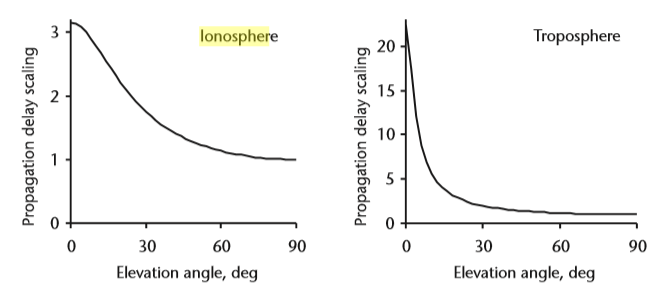
\includegraphics[scale=0.5]{bilder/groves_elev_atmo_error.png}
    \caption[Relation between atmospheric errors and elevation]{Atmospheric errors as a function of satellite elevation angle. (From \cite{groves2013principles})}
    \label{fig:atmo_elev_error}
\end{figure}

\subsubsection{Ephemeris error}
\label{sec:eph_error}
The ephemeris model is estimated through a curve fit to the measured orbit by the control segment and variations might therefore occur, \cite{farrell2008aided}. The result is a difference between actual and estimated SV position and the associated angle between actual and estimated signal path leads to a range error due to the long distance between receiver and SV. In fact, the sensitivity of position to the angular parameters in the ephemeris is in the order of $10^8 \deg$, while the angular rate parameters has a sensitivity in the order of $10^{12}deg/s$. \todo{citation needed}

\subsubsection{Multipath}
\label{sec:multipath}
Multipath errors occur when a satellite signal reach the receiver through multiple paths due to the signal reflecting off some surface. Signals that are reflected will arrive later than the signal taking the direct route and can usually be detected by the receiver if the delay is large enough. If the reflected signals arrive before the PRN code has been correlated however, interference can occur and shift the correlation peak. As the correlation peak is used to measure the delay from transmission to receival, pseudorange errors will occur. This also means that higher data rate signals are less susceptible to multipath errors \cite{groves2013principles}. \todo{verify}\\

Signals from satellites at low elevations travel nearly parallel to the surface of the Earth and the chance of the signal being reflected off the ground is therefore substantially higher. Thus, discarding data from these satellites might improve the GPS solution \cite{farrell2008aided, groves2013principles}.

\subsubsection{Group delay}
The clock correction polynomial, equation \ref{eq:eph_corr_time}, is incorporates the so called group delay of the GNSS equipment. This is the delay in the hardware of the satellite, from the initiation of a transmission until a signal is actually transmitted. However, the polynomial is tuned to dual frequency receivers, so single frequency receivers require an additional correction parameter \cite{spec:gps}. This is broadcast in the navigation message and applied as follows
\begin{equation}
    (\Delta t_{sv})_{L1C/A} = \Delta t_{sv} - T_{gd}
\end{equation}

For the modernized GPS, the civillian signals will include an additional correction called the \textit{inter-signal correction} \cite{spec:gps-new}.
%Delay between L1 and L2?


\subsubsection{Earth rotation: the Sagnac effect}
When working with the non-inertial ECEF frame, it is important to consider earth rotation during signal transmission. The ephemeris equations of \ref{sec:eph_equations} calculates satellite positions as a function of time, in the ECEF frame of that instant, while the receiver, on the other hand, estimates its position with respect to the ECEF frame at the time of signal reception. In other words, as illustrated in figure \ref{fig:sagnac}, the positions are expressed with respect to two separate coordinate frames. These must be aligned, as neglecting this may otherwise result in a significant east-west error of as much 41 meters at the equator \cite{groves2013principles}.\\

\begin{figure}[!htbp]
    \centering
    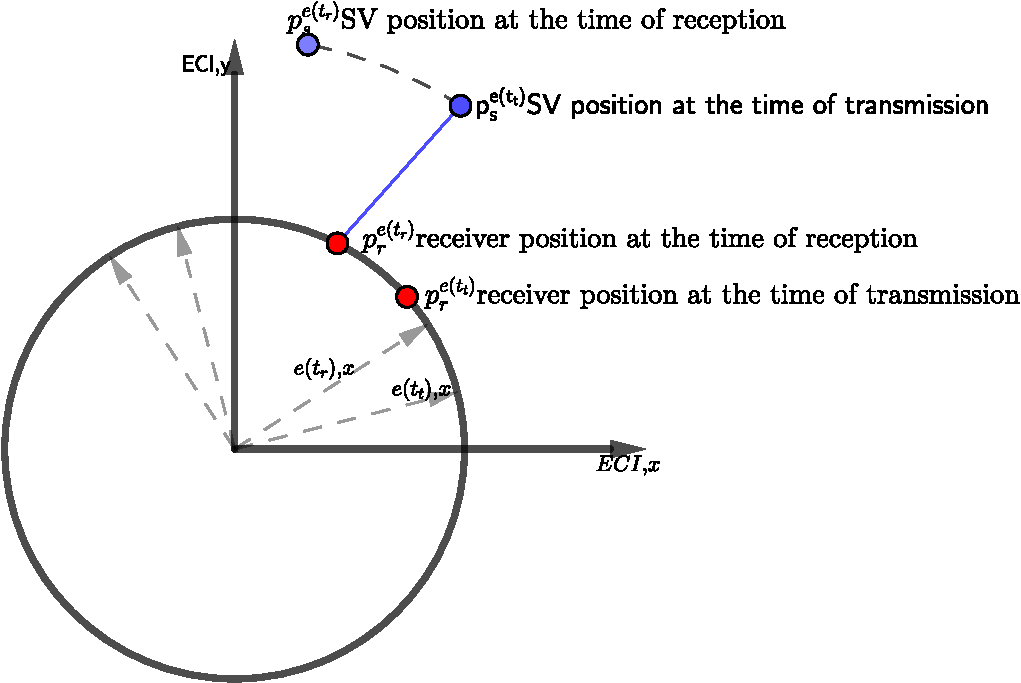
\includegraphics[scale=0.75]{bilder/sagnac.pdf}%{Theory/tikz/sagnac.tex}
    \caption{Illustration of earth rotation during signal transmission. }
    \label{fig:sagnac}
\end{figure}

Aligning either of the two frames with the other will be equivalent to using a single intertial frame \cite{groves2013principles}. The true range is then expressed as
\todo{Add to nomenclature/definitions}
\begin{align}
    \rho &= \norm{\bm{R}^{e(t_r)}_{e(t_t)}\bm{p}^{e(t_t)}_{s} - \bm{p}^{e(t_r)}_r}_2\\
\intertext{where the $t_r$ and $t_t$ denotes the time of reception and transmission respectively, $e(t_x)$ is the ECEF frame at time $t_x$ with respect to a common inertial frame and $\bm{R}^{e(t_r)}_{e(t_t)}$ is the rotation matrix from the satellite frame to the receiver frame. As the different frames share both origin and a single axis, the rotation matrix is given by}
    \bm{R}^{e(t_r)}_{e(t_t)} &= 
    \begin{bmatrix}
        cos(w_{ie}(t_r-t_t))  & sin(w_{ie}(t_r-t_t)) & 0\\
        -sin(w_{ie}(t_r-t_t)) & cos(w_{ie}(t_r-t_t)) & 0\\
        0                     & 0                    & 1
    \end{bmatrix}\\
\intertext{However, given the low rotation speed of the earth, in the order of $10^-5$, it is reasonable to apply the small angle approximation, $sin(\theta) = \theta$ and $cos(\theta) = 1$}
\bm{R}^{e(t_r)}_{e(t_t)} &\approx 
    \begin{bmatrix}
        1                   & w_{ie}(t_r-t_t)  & 0\\
        -w_{ie}(t_r-t_t)    & 1                & 0\\
        0                   & 0                & 1
    \end{bmatrix}
    =
    \begin{bmatrix}
        1                     & w_{ie}\frac{\rho}{c} & 0\\
        -w_{ie}\frac{\rho}{c} & 1                    & 0\\
        0                     & 0                    & 1
    \end{bmatrix}
\end{align}

It is also possible to approximate this effect as a correction term, often called the sagnac correction
\begin{align}
    \label{eq:range-sagnac}
    \rho &\approx \norm{\bm{p}^{e(t_t)}_{s} - \bm{p}^{e(t_r)}_r} + \delta\rho_{sagnac}\\
    \intertext{With the correction approximated to}
    \label{eq:sagnac-corr}
    \delta\rho_{sagnac} &\approx \frac{\omega_{ie}}{c}(y^{e(t_t)}_{s}x^{e(t_r)}_{r}-x^{e(t_t)}_{s}y^{e(t_r)}_{r})
\end{align}

The non-inertial frame will also affect the range rate measurements with an error of up to 2$\frac{mm}{s}$ \cite{groves2013principles}. This correction term is found by differentiating equation \ref{eq:sagnac-corr}.
\begin{equation}
    \delta\dot{\rho}_{sagnac} \approx \frac{\omega_{ie}}{c}(v^{e(t_t)}_{s}x^{e(t_r)}_{r} + u^{e(t_r)}_{r}y^{e(t_t)}_{s}-u^{e(t_t)}_{s}y^{e(t_r)}_{r}-x^{e(t_t)}_{s}v^{e(t_r)}_{r})
\end{equation}
\todo{Add this to definitions/nomenclature}
Where $u$ and $v$ denote the $x$ and $y$ component of receiver and satellite velocity vector.

\subsubsection{Relativistic errors}
Due to the high speeds and different gravity potential from the high orbit of the satellites, relativistic effects influences the satellite clock frequencies. This effect can be split into a constant frequency component from the satellite's nominal orbit, modified in factory, and a periodic frequency component due to the eccentricity of the orbit. The periodic component must be compensated for by the receiver, as described in section \ref{sec:ephemeris}, or it could lead to a worst case error of close to 13 meters, \cite{misra2006global}.\\

Without the constant frequency correction applied, the difference in observed frequencies would accumulate to a clock error of approximately $38 \mu s$ a day, equivalent to a navigation error of approximately 11 km \cite{pascual2007introducing}
